\documentclass[tikz,border=5pt]{standalone}
\usepackage{amsmath}
\usetikzlibrary{arrows.meta,3d}
\usepackage{tikz-3dplot}

% 样式与宏:集中定义以减少重复,保持原有视觉
\tikzset{
    edge visible/.style={gray,thin},
    edge hidden/.style={gray,thin,dashed},
    gridnode/.style={circle,fill=black,minimum size=4pt,inner sep=0pt},
    centernode/.style={circle,fill=green!60!black,minimum size=6pt,inner sep=0pt},
    dirarrow/.style={gray,->,line width=2pt,opacity=0.7},
    dirarrowfaint/.style={gray,->,line width=2pt,opacity=0.3},
    weightlabel/.style={blue,anchor=north east},
    dirnum/.style={red,font=\footnotesize},
    axisarrow/.style={black,->,line width=0.8pt},
    axisarrowX/.style={red!80!black,->,line width=0.9pt},
    axisarrowY/.style={green!60!black,->,line width=0.9pt},
    axisarrowZ/.style={blue!70!black,->, line width=0.9pt}
}

% 通用小工具宏:用于减少重复并保持锚点与样式一致
% 将权重批量放置到两组索引(奇/偶)处
% 参数:#1 odd 索引列表, #2 even 索引列表, #3 数学内容, #4 odd 锚点, #5 even 锚点
\newcommand{\PlaceWeights}[5]{%
    \foreach \i in #1 {\node[weightlabel,anchor=#4,yshift=1.5pt] at (P\i) {#3};}%
    \foreach \i in #2 {\node[weightlabel,anchor=#5,yshift=1.5pt] at (P\i) {#3};}%
}

% 按前缀批量放置方向编号(用于主图 P 和插图 Q)
% 参数:#1 odd 索引列表, #2 even 索引列表, #3 坐标前缀(P 或 Q)
\newcommand{\PlaceDirNumsAt}[3]{%
    \foreach \i in #1 {\node[dirnum,anchor=south west] at (#3\i) {\i};}%
    \foreach \i in #2 {\node[dirnum,anchor=south east] at (#3\i) {\i};}%
}

% 方向列表:保持与原图一致
\def\DIRECTIONS{
    1/0/0, -1/0/0, 0/1/0, 0/-1/0, 0/0/1, 0/0/-1,
    1/1/0, -1/1/0, 1/-1/0, -1/-1/0,
    1/0/1, -1/0/1, 1/0/-1, -1/0/-1,
    0/1/1, 0/-1/1, 0/1/-1, 0/-1/-1,
    1/1/1, -1/1/1, 1/-1/1, -1/-1/1,
    1/1/-1, -1/1/-1, 1/-1/-1, -1/-1/-1
}

% 索引组:用于统一控制权重标注、箭头样式和编号锚点(不改变视觉)
% 注意:TeX 控制序列名仅由字母组成,避免下划线带来的解析错误
% faces: 1..6; edges: 7..18; corners: 19..26
\def\IDXFACESODD{1,3,5}
\def\IDXFACESEVEN{2,4,6}
\def\IDXEDGESODD{7,9,11,13,15,17}
\def\IDXEDGESEVEN{8,10,12,14,16,18}
\def\IDXCORNERSODD{19,21,23,25}
\def\IDXCORNERSEVEN{20,22,24,26}
% x=0 平面(强箭头)与其余(淡箭头)
\def\IDXXZERO{3,4,5,6,15,16,17,18}
\def\IDXEXPLODED{1,2,7,8,9,10,11,12,13,14,19,20,21,22,23,24,25,26}
% 奇偶索引集合(用于编号锚点分配)
\def\IDXALLODD{1,3,5,7,9,11,13,15,17,19,21,23,25}
\def\IDXALLEVEN{2,4,6,8,10,12,14,16,18,20,22,24,26}

% 横向切片间距(投影后水平间距)
\def\slicegap{1.0}

\begin{document}
    % 主视角(若使用 tikz-3dplot 的投影样式,可启用下一行并在 tikzpicture 选项中加入 tdplot_main_coords)
    %\tdplotsetmaincoords{70}{120}
    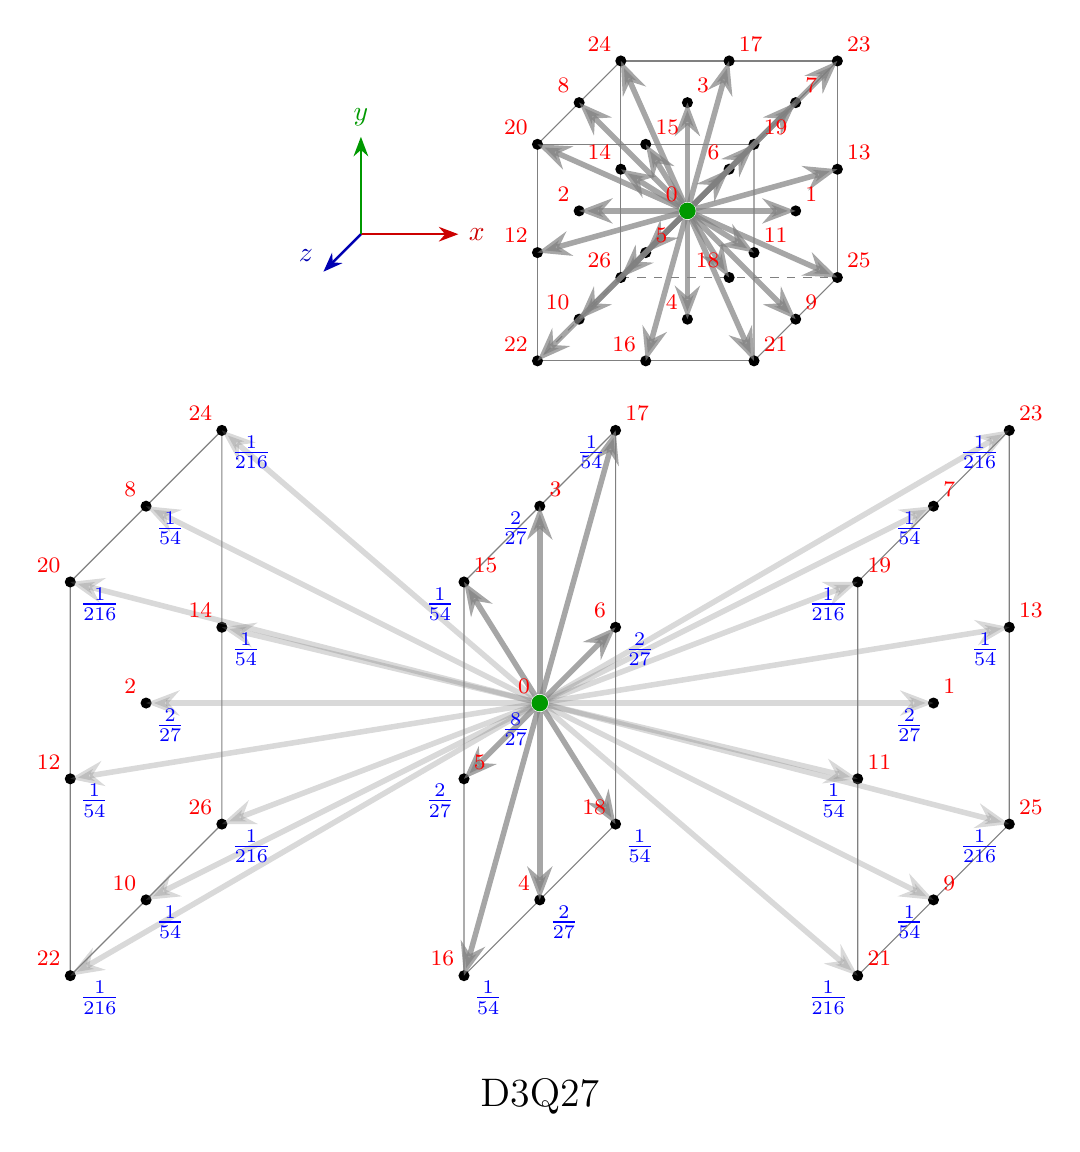
\begin{tikzpicture}[scale=2.5,>=Stealth]

    % draw the three x-planes as separate 3x3 grids
    \foreach \xp in {-1,0,1} {
        \pgfmathsetmacro{\dx}{\slicegap*\xp}
        \begin{scope}[shift={(\dx,0)}]
            % plane frame at x=\xp
            \draw[edge visible] (\xp,-1,-1) -- (\xp, 1,-1) -- (\xp, 1, 1) -- (\xp,-1, 1) -- cycle;
            % 9 grid nodes for this slice
            \foreach \y in {-1,0,1} {
                \foreach \z in {-1,0,1} {
                    \node[gridnode] at (\xp,\y,\z) {};
                }
            }
        \end{scope}
    }

    % center node (remains in the middle slice, unshifted)
    \node[centernode] (centerX) at (0,0,0) {};

    % create named endpoints for all 26 directions with per-slice horizontal shift
    \foreach [count=\i from 1] \x/\y/\z in \DIRECTIONS {
        \pgfmathsetmacro{\dx}{\slicegap*\x}
        \begin{scope}[shift={(\dx,0)}]
            \coordinate (P\i) at (\x,\y,\z);
        \end{scope}
    }

    % arrows from the center to each endpoint
    % strong arrows to same x-slice (x=0)
    \foreach \i in \IDXXZERO {\draw[dirarrow] (centerX) -- (P\i);}    
    % lighter arrows to exploded slices (x=±1)
    \foreach \i in \IDXEXPLODED {\draw[dirarrowfaint] (centerX) -- (P\i);}    

    % all weights (placed with opposite anchors to direction numbers to avoid overlap)
    % center
    \node[weightlabel] at (0,0,0) {$\frac{8}{27}$};

    % face centers (6) -> 2/27
    \PlaceWeights{\IDXFACESODD}{\IDXFACESEVEN}{$\frac{2}{27}$}{north east}{north west}

    % edges (12) -> 1/54
    \PlaceWeights{\IDXEDGESODD}{\IDXEDGESEVEN}{$\frac{1}{54}$}{north east}{north west}

    % corners (8) -> 1/216
    \PlaceWeights{\IDXCORNERSODD}{\IDXCORNERSEVEN}{$\frac{1}{216}$}{north east}{north west}

    % direction numbers (0-26)
    \node[dirnum,anchor=south east] at (0,0,0) {0};
    % 奇偶分组锚点保持与原图一致:奇数 SW,偶数 SE
    \PlaceDirNumsAt{\IDXALLODD}{\IDXALLEVEN}{P}

    % title
    \node[font=\Large] at (0,-2,0) {D3Q27};

    % =====================
    % Inset: full cube view
    % =====================
    % Place smaller overall cube centered above the exploded layout (closer vertically)
    \begin{scope}[shift={(0.75,2.5)}, scale=0.55]
        % 立方体框架
        \draw[edge hidden] (-1,-1,-1) -- (1,-1,-1);
        \draw[edge hidden] (-1,-1,-1) -- (-1,1,-1);
        \draw[edge hidden] (-1,-1,-1) -- (-1,-1,1);
        \draw[edge visible] (1,-1,-1) -- (1,1,-1) -- (-1,1,-1) -- (-1,-1,-1);
        \draw[edge visible] (1,-1,-1) -- (1,-1,1) -- (1,1,1) -- (1,1,-1);
        \draw[edge visible] (1,-1,1) -- (-1,-1,1) -- (-1,1,1) -- (1,1,1);
        \draw[edge visible] (-1,1,-1) -- (-1,1,1);
        \draw[edge visible] (-1,-1,1) -- (1,-1,1);
        \draw[edge visible] (1,1,-1) -- (1,1,1);

        % 3x3x3 网格节点
        \foreach \x in {-1,0,1} {
            \foreach \y in {-1,0,1} {
                \foreach \z in {-1,0,1} {
                    \node[gridnode] at (\x,\y,\z) {};
                }
            }
        }

        % 中心绿色节点 (0,0,0)
        \node[centernode] (center) at (0,0,0) {};

        % 26 个非中心方向端点(Q1..Q26)与箭头
        \foreach [count=\i from 1] \x/\y/\z in \DIRECTIONS {
            \coordinate (Q\i) at (\x,\y,\z);
            \draw[dirarrow] (center) -- (Q\i);
        }

    % 代表性权重(为避免遮挡,插图中不再显示)

    % 方向编号 0-26(奇 SW / 偶 SE)
        \node[dirnum,anchor=south east] at (0,0,0) {0};
    \PlaceDirNumsAt{\IDXALLODD}{\IDXALLEVEN}{Q}

        % 坐标轴:放在立方体左侧,标明 x,y,z 方向
    \coordinate (A0) at (-3.15,-0.35,-0.35);
    \draw[axisarrowX] (A0) -- ++(0.9,0,0) node[anchor=west, text=red!80!black] {$x$};
    \draw[axisarrowY] (A0) -- ++(0,0.9,0) node[anchor=south, text=green!60!black] {$y$};
    \draw[axisarrowZ] (A0) -- ++(0,0,0.9) node[anchor=south east, text=blue!70!black] {$z$};

        % 小标题(保持隐藏,避免与上方留白冲突)
        % \node[font=\large] at (0,-2,0) {D3Q27};
    \end{scope}

\end{tikzpicture}
\end{document}
